%!TEX root = ../larxxia.tex

\section{Geometry underlies determinants}
\label{sec:gud}
\secttoc

\begin{comment}
Develop {determinant}s from a geometric basis to most quickly get critical results.
This geometric approach ``encourages students to engage in what Blum and Kirsch call preformal proving'' \cite[p.401]{Hannah96}.
\end{comment}

Sections~\ref{sec:dmd}, \ref{sec:omr} and~\ref{sec:ilt} introduced that multiplication by a matrix transforms areas and volumes.
Determinants give precisely how much a square matrix transforms such areas and volumes.

\begin{example} \label{eg:detarea1}
Consider the square matrix \(A=\begin{bmatrix} \frac12&1\\0&1 \end{bmatrix}\).
Use matrix multiplication to find the image of the unit square under the transformation by~\(A\).
How much is the area of the unit square scaled up/down?  
Compare with the determinant.
\begin{solution} 
Consider the corner points of the unit square, under multiplication by~\(A\): 
\marginpar{\TwoD{0.5}101}%
using the `mapsto' symbol~\(\mapsto\) to denote that vector~\xv\ transforms to~\(A\xv\), \((0,0)\mapsto(0,0)\), \((1,0)\mapsto(\frac12,0)\), \((0,1)\mapsto(1,1)\), and \((1,1)\mapsto(\frac32,1)\), as shown in the marginal picture 
(the `roof' is only plotted to uniquely identify the sides).
The resultant parallelogram has area of~\(\frac12\) as its base is~\(\frac12\) and its height is~\(1\).
This parallelogram area of~\(\tfrac12\) is the same as the determinant since here~\eqref{eq:dets23b} gives \(\det A=\frac12\cdot1-0\cdot1=\frac12\)\,. 
\end{solution}
\end{example}


\begin{example} \label{eg:detarea2}
Consider the square matrix \(B=\begin{bmatrix} -1&1\\1&1 \end{bmatrix}\).
Use matrix multiplication to find the image of the unit square under the transformation by~\(B\).
How much is the unit area scaled up/down?  
Compare with the determinant.
\begin{solution} 
Consider the corner points of the unit square, under multiplication by~\(B\): 
\marginpar{\TwoD{-1}111}%
\((0,0)\mapsto(0,0)\), \((1,0)\mapsto(-1,1)\), \((0,1)\mapsto(1,1)\), and \((1,1)\mapsto(0,2)\), as shown in the marginal picture.
Through multiplication by the matrix~\(B\), the unit square is expanded, rotated and reflected.
The resultant square has area of~\(2\) as its sides are all of length~\(\sqrt2\).
This area has the same magnitude as the determinant since here~\eqref{eq:dets23b} gives \(\det B=(-1)\cdot1-1\cdot1=-2\)\,.
\end{solution}
\end{example}



\begin{activity}
Upon multiplication by the matrix~\(\begin{bmatrix} -2&5\\-3&-2 \end{bmatrix}\) the unit square transforms to a parallelogram.
Use the determinant of the matrix to find the area of the parallelogram is which of the following.
\partswidth=5em
\begin{parts}
\item \(4\)
\item \(11\)
\item \(16\)
\item \(19\)\actans
\end{parts}
\end{activity}



\begin{example} \label{eg:detarea3}
Consider the square matrix \(C=\begin{bmatrix} 2&0&0\\1&1&0\\0&0&\frac32 \end{bmatrix}\).
Use matrix multiplication to find the image of the unit cube under the transformation by~\(C\).
How much is the volume of the unit cube scaled up/down?  
Compare with the determinant.
\begin{solution} 
Consider the corner points of the unit cube under multiplication by~\(C\): \((0,0,0)\mapsto(0,0,0)\), \((1,0,0)\mapsto(2,1,0)\), \((0,1,0)\mapsto(0,1,0)\),  \((0,0,1)\mapsto(0,0,\frac32)\), and so on, as shown below (in stereo):
\begin{equation*}
\def\unithousesize{small}
\ThreeD20011000{1.5}
\end{equation*}
Through multiplication by the matrix~\(C\), the unit cube is deformed to a parallelepiped.
The resultant parallelepiped has volume of~\(3\) as it has height~\(\frac32\) and the parallelogram base has area~\(2\cdot1\).
This volume is the same  as the matrix determinant since~\eqref{eq:dets23b} gives \(\det G=2\cdot1\cdot\frac32+0+0-0-0-0=3\)\,.
\end{solution}
\end{example}






\Needspace{15\baselineskip}
\paragraph{Determinants determine area transformation}
Consider multiplication by the general \(2\times2\) matrix \(A=\begin{bmatrix} a&b\\c&d \end{bmatrix}\).

\begin{wrapfigure}{r}{0pt} 
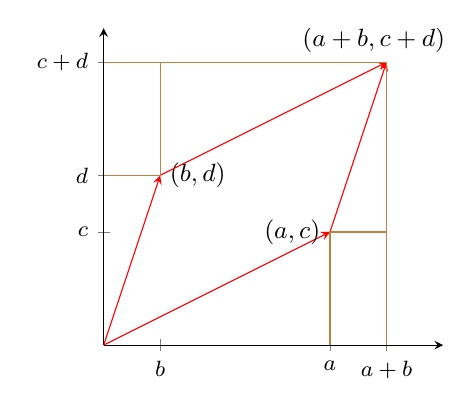
\begin{tikzpicture} 
\def\a{2} \def\b{0.5} \def\ab{2.5}
\def\c{1} \def\d{1.5} \def\cd{2.5}
\begin{axis}[axis equal image, axis lines=middle
    ,xtick={\a,\b,\ab},xticklabels={$a$,$b$,$a+b$}
    ,ytick={\c,\d,\cd},yticklabels={$c$,$d$,$c+d$}
    ,xmax=3,ymax=2.8,small
    ]
    \addplot[quiver={u=\a,v=\c},red,-stealth] coordinates {(0,0)};
    \node[left] at (axis cs:\a,\c) {\small$(a,c)$};
    \addplot[quiver={u=\b,v=\d},red,-stealth] coordinates {(0,0)};
    \node[right] at (axis cs:\b,\d) {\small$(b,d)$};
    \addplot[quiver={u=\a,v=\c},red,-stealth] coordinates {(\b,\d)};
    \addplot[quiver={u=\b,v=\d},red,-stealth] coordinates {(\a,\c)};
    \node[above] at (axis cs:\ab,\cd) {\small$(a+b,c+d)\quad$};
    \addplot[brown] coordinates {(\ab,0)(\ab,\cd)(0,\cd)};
    \addplot[brown] coordinates {(\ab,0)(\ab,\c)(\a,\c)(\a,0)};
    \addplot[brown] coordinates {(0,\cd)(\b,\cd)(\b,\d)(0,\d)};
\end{axis}
\end{tikzpicture}
\end{wrapfigure}
Under multiplication by this matrix~\(A\) the unit square becomes the parallelogram shown with four corners at \((0,0)\), \((a,c)\), \((b,d)\) and \((a+b,c+d)\).
Let's determine the area of the parallelogram by that of the containing rectangle less the two small rectangles and the four small triangles.
The two small rectangles have the same area, namely~\(bc\).
The two small triangles on the left and the right also have the same area, namely~\(\frac12bd\).
The two small triangles on the top and the bottom have the same area, namely~\(\frac12ac\).
Thus, under multiplication by matrix~\(A\) the image of the unit square is the parallelogram with 
\begin{eqnarray*}
\text{area}&=&(a+b)(c+d)-2bc-2\cdot\frac12bd-2\cdot\frac12ac
\\&=&ac+ad+bc+bd-2bc-bd-ac
\\&=&ad-bc=\det A\,.
\end{eqnarray*}
This picture is the case when the matrix does not also reflect the image:  if the matrix also reflects, as in Example~\ref{eg:detarea2}, then the determinant is the negative of the area.
In either case, the area of the unit square after transforming by the matrix~\(A\) is the magnitude~\(|\det A|\).


\Needspace{7\baselineskip}
\begin{wrapfigure}{r}{0pt}
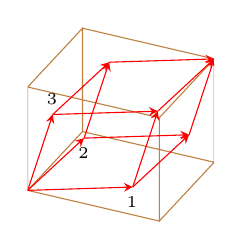
\begin{tikzpicture} 
\def\a{2.0} \def\b{0.5} \def\c{0.3} \def\ab{2.5}\def\ac{2.3}\def\bc{0.8}
\def\d{0.5} \def\e{1.5} \def\f{0.5} \def\de{2.0}\def\df{1.0}\def\ef{2.0}
\def\g{0.3} \def\h{0.5} \def\i{1.5} \def\gh{0.8}\def\gi{1.8}\def\hi{2.0}
\def\x{2.8}\def\y{2.5}\def\z{2.3}
%\def\o{0.3}%opacity
\begin{axis}[small,axis equal image
    ,hide x axis, hide y axis, hide z axis
    ]
    \addplot3[brown] coordinates {
    (0,0,0)(\x,0,0)(\x,\y,0)(0,\y,0)
    (0,0,0)(0,0,\z)(\x,0,\z)(\x,0,0)
    (0,0,0)(0,0,\z)(0,\y,\z)(0,\y,0)
    (0,\y,\z)(\x,\y,\z)(\x,0,\z)(\x,0,0)(\x,\y,0)(\x,\y,\z)
    };
%
    \addplot3[quiver={u=\a,v=\d,w=\g},red,-stealth] coordinates {(0,0,0)};
    \addplot3[quiver={u=\a,v=\d,w=\g},red,-stealth] coordinates {(\b,\e,\h)};
    \addplot3[quiver={u=\a,v=\d,w=\g},red,-stealth] coordinates {(\c,\f,\i)};
    \addplot3[quiver={u=\a,v=\d,w=\g},red,-stealth] coordinates {(\bc,\ef,\hi)};
    \node[below] at (axis cs:\a,\d,\g) {\footnotesize$\av_1$};
    \addplot3[quiver={u=\b,v=\e,w=\h},red,-stealth] coordinates {(0,0,0)};
    \addplot3[quiver={u=\b,v=\e,w=\h},red,-stealth] coordinates {(\a,\d,\g)};
    \addplot3[quiver={u=\b,v=\e,w=\h},red,-stealth] coordinates {(\c,\f,\i)};
    \addplot3[quiver={u=\b,v=\e,w=\h},red,-stealth] coordinates {(\ac,\df,\gi)};
    \node[below] at (axis cs:\b,\e,\h) {\footnotesize$\av_2$};
    \addplot3[quiver={u=\c,v=\f,w=\i},red,-stealth] coordinates {(0,0,0)};
    \addplot3[quiver={u=\c,v=\f,w=\i},red,-stealth] coordinates {(\a,\d,\g)};
    \addplot3[quiver={u=\c,v=\f,w=\i},red,-stealth] coordinates {(\b,\e,\h)};
    \addplot3[quiver={u=\c,v=\f,w=\i},red,-stealth] coordinates {(\ab,\de,\gh)};
    \node[above] at (axis cs:\c,\f,\i) {\footnotesize$\av_3$};
%    \addplot3[patch,opacity=\o,red]
%    coordinates {(\x+\s,-\h+\y,0+\t) (\x+\s,-\h+\y,\h+\t) (\x+\s,\h+\y,\h+\t)};
\end{axis}
\end{tikzpicture}
\end{wrapfigure}
Analogous geometric arguments relate determinants of \(3\times 3\) matrices with transformations of volumes.
Under multiplication by a \(3\times 3\) matrix~\(A=\begin{bmatrix} \av_1&\av_2&\av_3 \end{bmatrix}\), the image of the unit cube is a parallelepiped with edges~\(\av_1\), \(\av_2\) and~\(\av_3\) as illustrated.
By computing the volumes of various rectangular boxes, prisms and tetrahedra (or by other methods), 
the volume of such a parallelepiped could be expressed as the \(3\times3\) {determinant} formula~\eqref{eq:dets23b}.

In higher dimensions we want the determinant to behave analogously and so next define the determinant to do so.
We use the terms \index{nD-cube@$n$D-cube|textbf}\textbf{$n$D-cube} to generalise a square and cube to \(n\)~dimensions (\(\RR^n)\), \index{nD-volume@$n$D-volume|textbf}\textbf{$n$D-volume} to generalise the notion of area and volume to \(n\)~dimensions, and so on.
When the dimension of the space is unspecified, then we may say \bfidx{hyper-cube}, \bfidx{hyper-volume}, and so on.


\begin{definition} \label{def:detarea} 
Let \(A\) be an \(n\times n\) \idx{square matrix}, and let \(C\)~be the unit \index{nD-cube@$n$D-cube}$n$D-cube in~\(\RR^n\).
Transform the \(n\)D-cube~\(C\) by \(\xv\mapsto A\xv\) to its image~\(C'\) in~\(\RR^n\). 
Define the \bfidx{determinant} of~\(A\), denoted either~\(\det A\) or sometimes~\(|A|\) such that:  \begin{itemize}
\item the magnitude~\(|\det A|\) is the \index{nD-volume@$n$D-volume}$n$D-volume of~\(C'\); and 
\item the sign of~\(\det A\) to be negative iff the transformation reflects the orientation of the $n$D-cube.
\end{itemize}
\end{definition}




\begin{example} \label{eg:}
Roughly estimate the determinant of the matrix that transforms the unit square to the parallelogram as shown in the margin.
\marginpar{\TwoD{-0.7}0{1}{0.8}}
\begin{solution} 
The image is a parallelogram with a vertical base of length about~\(0.8\) and a horizontal height of about~\(0.7\) so the area of the image is about~\(0.8\times0.7=0.56\approx 0.6\)\,.
But the image has been reflected as one cannot rotate and stretch to get the image (remember the origin is fixed under matrix multiplication): thus the determinant must be negative.
Our estimate for the matrix determinant is~\(-0.6\)\,.
\end{solution}
\end{example}



\begin{activity}
Roughly estimate the determinant of the matrix that transforms the unit square to the rectangle as shown in the margin.
\marginpar{\TwoD{1.2}{1.2}{-0.9}{1.6}}
\partswidth=5em
\begin{parts}
\item \(2\)
\item \(2.5\)
\item \(3\)\actans
\item \(4\)
\end{parts}
\end{activity}




Basic properties of a determinant follow direct from Definition~\ref{def:detarea}.


\begin{theorem} \label{thm:basicdet}
\begin{enumerate}
\item \label{thm:basicdet:i}  Let \(D\) be an \(n\times n\) \idx{diagonal matrix}.
The \idx{determinant} of~\(D\) is the product of the diagonal entries: \(\det D=d_{11}d_{22}\cdots d_{nn}\)\,.
\item \label{thm:basicdet:ii} An \idx{orthogonal matrix}~\(Q\) has  \(\det Q=\pm1\) (only one alternative, not both), and \(\det Q=\det(\tr Q)\).
\item \label{thm:basicdet:iii}  For an \(n\times n\) matrix~\(A\), \(\det(kA)=k^n\det A\) for every scalar~\(k\).
\end{enumerate}
\end{theorem}
\begin{proof} Use Definition~\ref{def:detarea}.
%Direct from definition, and that an orthogonal matrix is a rotation and so preserves $n$D-volumes (\(\det Q=\det(\tr Q)=-1\) if \(Q\)~also involves a reflection).
\begin{itemize}
\Needspace{8\baselineskip}
\item[\ref{thm:basicdet:i}.]
The unit $n$D-cube in~\(\RR^n\) has edges \hlist\ev n\ (the unit vectors).
Multiplying each of these edges by the diagonal matrix \(D=\diag(d_{11},d_{22},\ldots,d_{nn})\) maps the unit $n$D-cube to a $n$D-`rectangle' with edges \(d_{11}\ev_1,d_{22}\ev_2,\ldots,d_{nn}\ev_n\) (as illustrated in the margin).
\marginpar{\def\unithouseviews{30}\ThreeD30002000{0.5}}
Being a $n$D-rectangle with all edges orthogonal, its $n$D-volume is the product of the length of the sides; that is, \(|\det D|=|d_{11}|\cdot|d_{22}|\cdots |d_{nn}|\).
The $n$D-cube is reflected only if there are an odd number of negative diagonal elements, hence the sign of the determinant is such that \(\det D=d_{11}d_{22}\cdots d_{nn}\)\,.

\item[\ref{thm:basicdet:ii}.]
Multiplication by an orthogonal matrix~\(Q\) is a rotation and/or reflection as it preserves all lengths and angles (Theorem~\ref{thm:orthog:iv}).
Hence it preserves $n$D-volumes.
Consequently the image of the unit $n$D-cube under multiplication by~\(Q\) has the same volume of one; that is, \(|\det Q|=1\)\,.
The sign of~\(\det Q\) characterises whether multiplication by~\(Q\) has a reflection.

When \(Q\)~is orthogonal then so is~\(\tr Q\) (Theorem~\ref{thm:orthog:ia}).  Hence \(\det\tr Q=\pm1\)\,.
Multiplication by~\(Q\) involves a reflection iff its inverse of multiplication by~\(\tr Q\) involves the reflection back again.
Hence the signs of the two determinants must be the same: that is, \(\det Q=\det\tr Q\)\,.

\item[\ref{thm:basicdet:iii}.]
Let the matrix~\(A\) transform the unit $n$D-cube to a $n$D-parallelepiped~\(C'\) that  (by definition) has $n$D-volume~\(|\det A|\).
Multiplication by the matrix~\((kA)\) then forms a $n$D-parallelepiped which is \(|k|\)-times bigger than~\(C'\) in every direction.
In~\(\RR^n\) its $n$D-volume is then \(|k|^n\)-times bigger; that is,
\(|\det(kA)|=|k|^n|\det A|=|k^n\det A|\).
If the scalar~\(k\) is negative then the orientation of the image is reversed (reflected) only in odd~\(n\) dimensions; that is, the sign of the determinant is multiplied by~\((-1)^n\).
\marginpar{\TwoD{-1}00{-1}}%
(For example, the unit square shown in the margin is transformed through multiplication by~\((-1)I_2\) and the effect is the same as rotation by~\(180^\circ\), without any reflection as \((-1)^2=1\)\,.)
Hence for all real~\(k\), the orientation is such that \(\det(kA)=k^n\det A\). 
\end{itemize}
\end{proof}

\begin{example} \label{eg:detident}
The determinant of the \(n\times n\) identity matrix is one: that is, \(\det I_n=1\)\,. 
We justify this result in two ways.
\begin{itemize}
\item An identity matrix is a diagonal matrix and hence its determinant is the product of the diagonal entries (Theorem~\ref{thm:basicdet:i}) here all ones. 
\item Alternatively, multiplication by the identity does not change the unit $n$D-cube and so does not change its $n$D-volume (Definition~\ref{def:detarea}).
\end{itemize}
%The determinant of~\(-I_n\) is~\((-1)^n\) either by the product of the diagonals  (Theorem~\ref{thm:basicdet:i}), or because of the scalar multiplication Theorem~\ref{thm:basicdet:iii}.
\end{example}





\begin{activity}
What is the determinant of \(-I_n\)?
\begin{parts}
\item \(-1\)
\item \(+1\)
\item \(-1\) for odd~\(n\), and \(+1\) for even~\(n\) \actans
\item \(+1\) for odd~\(n\), and \(-1\) for even~\(n\)
\end{parts}
\end{activity}






\begin{example} \label{eg:}
Use~\eqref{eq:dets23b} to compute the determinant of the orthogonal matrix
\begin{equation*}
Q=\begin{bmatrix} \frac13&-\frac23&\frac23
\\\frac23&\frac23&\frac13
\\-\frac23&\frac13&\frac23 \end{bmatrix}.
\end{equation*}
Then use Theorem~\ref{thm:basicdet} to deduce the determinants of the following matrices:
\begin{equation*}
\begin{bmatrix} \frac13&\frac23&-\frac23
\\-\frac23&\frac23&\frac13
\\\frac23&\frac13&\frac23 \end{bmatrix}
,\quad
\begin{bmatrix} -1&2&-2
\\-2&-2&-1
\\2&-1&-2 \end{bmatrix}
,\quad
\begin{bmatrix} \frac16&-\frac13&\frac13
\\\frac13&\frac13&\frac16
\\-\frac13&\frac16&\frac13 \end{bmatrix}.
\end{equation*}

\begin{solution} 
\begin{itemize}
\item Using~\eqref{eq:dets23b} the determinant
\begin{eqnarray*}
\det Q&=&\tfrac13\tfrac23\tfrac23+(-\tfrac23)\tfrac13(-\tfrac23)
+\tfrac23\tfrac23\tfrac13
\\&&{}-\tfrac23\tfrac23(-\tfrac23)
-\tfrac13\tfrac13\tfrac13-(-\tfrac23)\tfrac23\tfrac23
\\&=&\tfrac1{27}(4+4+4+8-1+8)=1\,.
\end{eqnarray*}

\item The first matrix is~\(\tr Q\) for which \(\det\tr Q=\det Q=1\)\,.

\item The second matrix is minus three times~\(Q\) so, being \(3\times3\) matrices, its determinant is~\((-3)^3\det Q=-27\)\,.

\item The third matrix is half of~\(Q\) so, being \(3\times3\) matrices, its determinant is~\((\tfrac12)^3\det Q=\frac18\)\,.
\end{itemize}
\end{solution}
\end{example}



\begin{activity}
Given
\(\det\begin{bmatrix} 1&-1&-2&0
\\1&1&1&1
\\1&-1&-2&-1
\\-1&0&0&-1 \end{bmatrix}=-1\)\,,
what is 
\(\det\begin{bmatrix} -2&2&4&0
\\-2&-2&-2&-2
\\-2&2&4&2
\\2&0&0&2 \end{bmatrix}\)?
\partswidth=5em
\begin{parts}
\item \(8\)
\item \(2\)
\item \(-4\)
\item \(-16\)
\end{parts}
\end{activity}


A consequence of Theorem~\ref{thm:basicdet:iii} is that a determinant characterises the transformation of any sized \idx{hyper-cube}. 
Consider the transformation by a matrix~\(A\) of an \index{nD-cube@$n$D-cube}$n$D-cube of side length~\(k\,(k\geq0)\).
The $n$D-cube has edges \hlist{k\ev}n.
The transformation results in an \index{nD-parallelepiped@$n$D-parallelepiped}$n$D-parallelepiped with edges \(A(k\ev_1),A(k\ev_2),\ldots,A(k\ev_n)\), which by commutativity and associativity (Theorem~\ref{thm:pmmc}) are the same edges as \hlist{(kA)\ev}n.
That is, the resulting $n$D-parallelepiped is the same as applying matrix~\((kA)\) to the unit $n$D-cube, and so must have \index{nD-volume@$n$D-volume}$n$D-volume~\(k^n|\det A|\).
Crucially, this property that matrix multiplication multiplies all sizes of hyper-cubes by the determinant holds for all other shapes and sizes, not just hyper-cubes.
Let's see an specific example before proving the general theorem.

\begin{example} \label{eg:}
Multiplication by some specific matrix transforms the (blue) triangle~\(C\) to the (red) triangle~\(C'\) as shown in the margin.  By finding the ratio of the areas, estimate the magnitude of the determinant of the matrix.
\marginpar{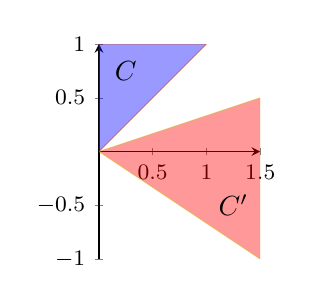
\begin{tikzpicture}
    \begin{axis}[footnotesize,axis equal image, axis lines=middle]
    \addplot[patch,fill=blue,opacity=0.4] coordinates {(0,0)(0,1)(1,1)};
    \node at (axis cs:0.25,0.75) {$C$};
    \addplot[patch,fill=red ,opacity=0.4] coordinates {(0,0)(1.5,0.5)(1.5,-1)};
    \node at (axis cs:1.25,-0.5) {$C'$};
    \end{axis}
\end{tikzpicture}}
\begin{solution} 
The (blue) triangle~\(C\) has vertical height one and horizontal base one, so has area~\(0.5\)\,.
The mapped (red) triangle~\(C'\) has vertical base of~\(1.5\) and horizontal height of~\(1.5\) so its area is~\(\frac12\times1.5\times1.5=1.25\)\,.
The mapped area is thus \(1.25/0.5=2.5\)~times bigger than the initial area; hence the determinant of the transformation matrix has magnitude \(|\det A|=2.5\)\,.

We cannot determine the sign of the determinant as we do not know about the orientation of~\(C'\) relative to~\(C\).
\end{solution}
\end{example}



\begin{theorem} \label{thm:detanyC} 
Consider any \idx{bounded} smooth \index{nD-volume@$n$D-volume}$n$D-volume~\(C\) in~\(\RR^n\) and its image~\(C'\) after multiplication by \(n\times n\) matrix~\(A\).
Then
\begin{equation*}
\det A=\pm\frac{\text{$n$D-volume of }C'}
{\text{$n$D-volume of }C}
\end{equation*}
with the negative sign when matrix~\(A\) changes the orientation.
\end{theorem}
\begin{proof} 
A proof is analogous to integration in calculus \cite[p.402]{Hannah96}. 
\marginpar{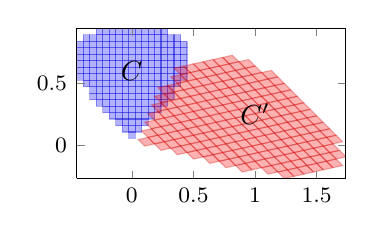
\begin{tikzpicture} 
\begin{axis}[footnotesize,axis equal image
    ,view={0}{90},restrict z to domain=0.5:2.5
    ,domain=-0.5:0.5,y domain=0:1]
    \addplot3[surf, samples=20, opacity=0.3]
        ({x},{y},{(x^2-y^2+y^4<0)});
    \node at (axis cs:0,0.6,1) {$C$};
    \addplot3[surf, samples=20, opacity=0.3]
        ({x+1.5*y},{-x+y/3},{2*(x^2-y^2+y^4<0)});
    \node at (axis cs:1,0.25,1) {$C'$};
\end{axis}
\end{tikzpicture}}
In two dimensions, as drawn in the margin,  we divide a given region~\(C\) into  many small squares of side length~\(k\), each of area~\(k^2\):  each of these transforms to a small parallelogram of area~\(k^2|\det A|\) (by Theorem~\ref{thm:basicdet:iii}), then the sum of the transformed areas is just \(|\det A|\)~times the  original area of~\(C\).

In  \(n\)-dimensions, divide a given region~\(C\) into  many small $n$D-cubes of side length~\(k\), each of $n$D-volume~\(k^n\):  each of these transforms to a small $n$D-parallelepiped of $n$D-volume~\(k^n|\det A|\) (by Theorem~\ref{thm:basicdet:iii}), then the sum of the transformed $n$D-volume is just \(|\det A|\)~times the  $n$D-volume of~\(C\). 
\end{proof}

A more rigorous proof would involve upper and lower sums for the original and transformed regions, and also explicit restrictions to regions where these upper and lower sums converge to a unique $n$D-volume. 
We do not detail such a more rigorous proof here.


This property of transforming general areas and volumes also establishes the next crucial property of determinants, namely that the determinant of a matrix product is the product of the determinants: \(\det(AB)=\det(A)\det(B)\) for all square matrices~\(A\) and~\(B\) (of the same size).

\begin{example} \label{eg:}
Recall the two \(2\times2\) matrices of Examples~\ref{eg:detarea1} and~\ref{eg:detarea2}:
\begin{equation*}
A=\begin{bmatrix} \frac12&1\\0&1 \end{bmatrix},\quad
B=\begin{bmatrix} -1&1\\1&1 \end{bmatrix}.
\end{equation*}
Check that the determinant of their product is the product of their determinants. 
\begin{solution} 
First, Examples~\ref{eg:detarea1} and~\ref{eg:detarea2} computed \(\det A=\tfrac12\) and \(\det B=-2\)\,.
Thus the product of their determinants is \(\det(A)\det(B)=-1\)\,.

Secondly, calculate the matrix product
\marginpar{\TwoD{0.5}{1.5}11}%
\begin{equation*}
AB=\begin{bmatrix} \frac12&1\\0&1 \end{bmatrix}
\begin{bmatrix} -1&1\\1&1 \end{bmatrix}
=\begin{bmatrix} \frac12&\frac32\\1&1 \end{bmatrix},
\end{equation*}
whose multiplicative action upon the unit square is illustrated in the margin.
By~\eqref{eq:dets23b}, \(\det(AB)=\frac12\cdot1-\frac32\cdot1=-1\)\,, as required.
 
Thirdly, we should also check the other product (as the question does not specify the order of the product):
\marginpar{\TwoD{-0.5}{0}{0.5}2}%
\begin{equation*}
BA=\begin{bmatrix} -1&1\\1&1 \end{bmatrix}
\begin{bmatrix} \frac12&1\\0&1 \end{bmatrix}
=\begin{bmatrix} -\frac12&0\\\frac12&2 \end{bmatrix},
\end{equation*}
whose multiplicative action upon the unit square is illustrated in the margin.
By~\eqref{eq:dets23b}, \(\det(BA)=-\frac12\cdot2-0\cdot\frac12=-1\)\,, as required.
\end{solution}
\end{example}



\begin{theorem} \label{thm:detprod} 
For every two \index{square matrix}\(n\times n\) matrices \(A\) and~\(B\), \(\det(AB)=\det(A)\det(B)\).
Further, for \(n\times n\) matrices \hlist A\ell, \(\det(A_1A_2\cdots A_\ell)=\det(A_1)\det(A_2)\cdots\det(A_\ell)\).
\end{theorem}


\begin{proof}  
Consider the unit $n$D-cube~\(C\),  its image~\(C'\) upon transforming by~\(B\), and the image~\(C''\) after transforming~\(C'\) by~\(A\). 
That is, each edge~\(\ev_j\) of cube~\(C\) is mapped to the edge~\(B\ev_j\) of~\(C'\), which is in turn mapped to edge~\(A(B\ev_j)\) of~\(C''\). 
By Definition~\ref{def:detarea}, \(C'\) has (signed) $n$D-volume~\(\det B\)\,.
Theorem~\ref{thm:detanyC} implies \(C''\) has (signed) $n$D-volume \(\det A\)~times that of~\(C'\); that is, \(C''\) has (signed) $n$D-volume~\(\det(A)\det(B)\).  

By associativity, the \(j\)th edge~\(A(B\ev_j)\) of~\(C''\) is the same as~\((AB)\ev_j\) and so \(C''\) is the image of~\(C\) under the transformation by matrix~\((AB)\).
Consequently, the (signed) $n$D-volume of~\(C''\) is alternatively given by~\(\det(AB)\).
These two expressions for the $n$D-volume of~\(C''\) must be equal: that is, \(\det(AB)=\det(A)\det(B)\).

Exercise~\ref{ex:detprodk} uses induction to then prove the second statement in the theorem that \(\det(A_1A_2\cdots A_\ell)=\det(A_1)\det(A_2)\cdots\det(A_\ell)\).
\end{proof}



\begin{activity}
Given that the matrices
%a=round(randn(3))+0,det(a)
\begin{equation*}
\begin{bmatrix} -1&0&-1
\\0&-1&1
\\0&1&1 \end{bmatrix},\quad
\begin{bmatrix} 0&1&-2
\\-1&-1&1
\\-1&-2&-1 \end{bmatrix},\quad
\begin{bmatrix} -1&0&-1
\\0&1&1
\\1&2&0 \end{bmatrix},
\end{equation*}
have determinants~\(2\)\,, \(-4\) and~\(3\), respectively, what is the determinant of the product of the three matrices?
\partswidth=5em
\begin{parts}
\item \(-24\)
\item \(1\)
\item \(9\)
\item \(24\)
\end{parts}
\end{activity}




\begin{example} \label{eg:}
\begin{enumerate}
\item\label{eg:baddets} Confirm the product rule for determinants, Theorem~\ref{thm:detprod}, for the product
\begin{equation*}
\begin{bmatrix} -3&-2\\3&-3 \end{bmatrix}
=\begin{bmatrix} 3&1&1\\0&-3&0 \end{bmatrix}
\begin{bmatrix} -1&0\\-1&1\\1&-3 \end{bmatrix}.
\end{equation*}
\begin{solution} 
Although the determinant of the left-hand matrix is \((-3)(-3)-3(-2)=9-(-6)=15\)\,, we cannot confirm the product rule because it does not apply: the matrices on the right-hand side are not square matrices and so do not have determinants.
\end{solution}

\item Given \(\det A=2\) and \(\det B=\pi\)\,, what is \(\det(AB)\)?
\begin{solution} 
Strictly, there is no answer as we do not know that matrices~\(A\) and~\(B\) are of the same size.
However, if we are \emph{additionally} given that \(A\) and~\(B\) are the same size, then Theorem~\ref{thm:detprod} gives \(\det(AB)=\det(A)\det(B)=2\pi\)\,.
\end{solution}
\end{enumerate}
\end{example}



\begin{example} \label{eg:}
Use the product theorem to help find the determinant of matrix
\begin{equation*}
C=\begin{bmatrix} 45&-15&30\\
-2\pi&\pi&2\pi\\
\frac19&\frac29&-\frac13 \end{bmatrix}.
\end{equation*}
\begin{solution} 
One route is to observe that there is a common factor in each row of the matrix so it may be factored as
\begin{equation*}
C=\begin{bmatrix} 15&0&0\\0&\pi&0\\0&0&\frac19 \end{bmatrix}
\begin{bmatrix} 3&-1&2\\-2&1&2\\1&2&-3 \end{bmatrix}.
\end{equation*}
The first matrix, being diagonal, has determinant that is the product of its diagonal elements (Theorem~\ref{thm:basicdet:i}) so its determinant\({}=15\pi\frac19=\frac53\pi\).
The second matrix, from~\eqref{eq:dets23b}, has determinant\({}=-9-2-8-2-12+6=-27\)\,.
Theorem~\ref{thm:detprod} then gives \(\det C=\frac53\pi\cdot(-27)=-45\pi\)\,.
\end{solution}
\end{example}



Recall that Theorem~\ref{thm:basicdet:ii} establishes that transposing an orthogonal matrix does not change its determinant, \(\det\tr Q=\det Q\)\,.
We now establish that this property holds for the transpose of all square matrices.


\begin{example} \label{eg:}
Example~\ref{eg:baddets} determined that
\(\det\begin{bmatrix} -3&-2\\3&-3 \end{bmatrix}=15\)\,.
By~\eqref{eq:dets23b}, its transpose has determinant
\begin{equation*}
\det\begin{bmatrix} -3&3\\-2&-3 \end{bmatrix}
=(-3)^2-3(-2)=9+6=15\,.
\end{equation*}
The determinants are the same.
\end{example}




\begin{theorem} \label{thm:dettr} 
For every \idx{square matrix}~\(A\), \(\det(\tr A)=\det A\).
\end{theorem}
\begin{proof} 
Use an \svd\ of the matrix, say \(A=\usv\).
Then 
\begin{eqnarray*}
\det A&=&\det(\usv)
\\&=&\det(U)\det(S)\det(\tr V)\quad(\text{by Theorem~\ref{thm:detprod}})
\\&=&\det(\tr U)\det(S)\det(V)\quad(\text{by Theorem~\ref{thm:basicdet:ii}})
\\&=&\det(\tr U)(\sigma_1\sigma_2\cdots\sigma_n)\det(V)\quad(\text{by Theorem~\ref{thm:basicdet:i}})
\\&=&\det(\tr U)\det(\tr S)\det(V)\quad(\text{by Theorem~\ref{thm:basicdet:i}})
\\&=&\det(V)\det(\tr S)\det(\tr U)\quad(\text{by scalar commutativity})
\\&=&\det(V\tr S\tr U)\quad(\text{by Theorem~\ref{thm:detprod}})
\\&=&\det[\tr{(\usv)}]=\det(\tr A).
\end{eqnarray*}
\end{proof}

\begin{example} \label{eg:}
A general \(3\times 3\) matrix \(A=\begin{bmatrix} a&b&c\\d&e&f\\g&h&i \end{bmatrix}\) has \idx{determinant} \(\det A=|A|=aei+bfg+cdh-ceg-afh-bdi\)\,.
Its transpose, \(\tr A=\begin{bmatrix} a&d&g\\b&e&h\\c&f&i \end{bmatrix}\), from the rule~\eqref{eq:dets23b}
\begin{equation*}
\setlength{\unitlength}{1ex}
\def\z{\hspace*{-0.15em}&}
\begin{picture}(16,9)
%\put(0,0){\framebox(16,9){}}
\put(0,4){\(\begin{bmatrix} a\z d\z g\\b\z e\z h\\c\z f\z i \end{bmatrix}
\begin{matrix} a\z b\\d\z e\\g\z h \end{matrix}\)
}
%\thicklines
\color{red}\multiput(2.1,1)(2.6,0)3{\line(1,1)7}
\color{blue}\multiput(2.0,8)(2.6,0)3{\line(1,-1)7}
\end{picture}
\end{equation*}
has determinant
\begin{equation*}
\det\tr A=aei+dhc+gbf-gec-ahf-dbi =\det A\,.
\end{equation*}
\end{example}



Since the proof of Theorem~\ref{thm:dettr} invoked the \svd\ of the matrix, we now proceed to link the determinant of a matrix to the singular values of the matrix.

\begin{example} \label{eg:}
Recall Example~\ref{eg:3by3svd} showed that the following matrix has the given \svd:
\begin{eqnarray*}
A&=&\begin{bmatrix}-4&-2&4
\\-8&-1&-4
\\6&6&0\end{bmatrix}
\\&=&\begin{bmatrix} \frac13&-\frac23&\frac23
\\\frac23&\frac23&\frac13
\\-\frac23&\frac13&\frac23 \end{bmatrix}
\begin{bmatrix} 12&0&0\\0&6&0\\0&0&3 \end{bmatrix}
\tr{\begin{bmatrix} -\frac89&-\frac19&-\frac49
\\-\frac49&\frac49&\frac79
\\-\frac19&-\frac89&\frac49 \end{bmatrix}}.
\end{eqnarray*}
Use this \svd\ to find the magnitude~\(|\det A|\).
\begin{solution} 
Given the \svd\ \(A=\usv\), the Product Theorem~\ref{thm:detprod} gives \(\det A=\det(U)\det(S)\det(\tr V)\).
\begin{itemize}
\item \(\det U=\pm1\) by Theorem~\ref{thm:basicdet:ii} as \(U\)~is an orthogonal matrix.
\item Using the Transpose Theorem~\ref{thm:dettr}, \(\det(\tr V)=\det V=\pm1\) as \(V\)~is orthogonal.
\item Since \(S=\diag(12,6,3)\) is diagonal, Theorem~\ref{thm:basicdet:i} asserts its determinant is the product of the diagonal elements; that is, \(\det S=12\cdot6\cdot3=216\)\,.
\end{itemize}
Consequently \(\det A=(\pm1)216(\pm1)=\pm216\)\,, so \(|\det A|=216\)\,.
\end{solution}
\end{example}






\begin{theorem} \label{thm:detsvd}
For every \(n\times n\) \idx{square matrix}~\(A\), the magnitude of its determinant \(|\det A|=\sigma_1\sigma_2\cdots\sigma_n\)\,, the product of all its \idx{singular value}s.
\end{theorem}

\begin{proof} 
Consider an \svd\ of the matrix \(A=\usv\).
Theorems~\ref{thm:basicdet} and~\ref{thm:detprod} empowers the following identities:
\begin{eqnarray*}
\det A&=&\det(\usv)
\\&=&\det(U)\det(S)\det(\tr V)
\quad(\text{by Theorem~\ref{thm:detprod}})
\\&=&(\pm 1)\det(S)(\pm 1)
\quad(\text{by Theorem~\ref{thm:basicdet:ii}})
\\&=&\pm \det S
\quad(\text{and since \(S\) is diagonal})
\\&=&\pm \sigma_1\sigma_2\cdots\sigma_n\,.
\quad(\text{by Theorem~\ref{thm:basicdet:i}})
\end{eqnarray*}
Hence \(|\det A|=\sigma_1\sigma_2\cdots\sigma_n\)\,.
\end{proof}

\begin{example} \label{eg:}
Confirm Theorem~\ref{thm:detsvd} for the matrix \(A=\begin{bmatrix} 10&2\\5&11 \end{bmatrix}\) of Example~\ref{eg:2by2svd}.
\begin{solution} 
Example~\ref{eg:2by2svd} gave the \svd
\begin{equation*}
\begin{bmatrix} 10&2\\5&11 \end{bmatrix}=
\begin{bmatrix} \frac35&-\frac45\\\frac45&\frac35 \end{bmatrix}
\begin{bmatrix} 10\sqrt2&0\\0&5\sqrt2 \end{bmatrix}
\tr{\begin{bmatrix} \frac1{\sqrt2}&-\frac1{\sqrt2}\\ \frac1{\sqrt2}&\frac1{\sqrt2} \end{bmatrix}},
\end{equation*}
so Theorem~\ref{thm:detsvd} asserts \(|\det A|=10\sqrt2\cdot5\sqrt 2=100\)\,.
Using~\eqref{eq:dets23b} directly, \(\det A=10\cdot11-2\cdot 5=110-10=100\) which agrees with the product of the singular values.
\end{solution}
\end{example}






\begin{activity}
%U=[1,-2,2;2,2,1;-2,1,2]/3
%S=[9,0,0;0,9,0;0,0,0]
%V=[-8,-1,-4;-4,4,7;-1,-8,4]/9
The matrix
\(A=\begin{bmatrix} -2&-4&5
\\-6&0&-6
\\5&4&-2 \end{bmatrix}\)
has an \svd\ of
\begin{equation*}
A=\begin{bmatrix} \frac13&-\frac23&\frac23
\\\frac23&\frac23&\frac13
\\-\frac23&\frac13&\frac23 \end{bmatrix}
\begin{bmatrix} 9&0&0\\0&9&0\\0&0&0 \end{bmatrix}
\tr{\begin{bmatrix} -\frac89&-\frac19&-\frac49
\\-\frac49&\frac49&\frac79
\\-\frac19&-\frac89&\frac49 \end{bmatrix}}.
\end{equation*}
What is the the magnitude of the determinant of~\(A\), \(|\det A\,|\)\,?
\partswidth=5em
\begin{parts}
\item \(0\) \actans
\item \(4\)
\item \(18\)
\item \(81\)
\end{parts}
\end{activity}




\begin{example} \label{eg:}
Use an \svd\ of the following matrix to find the magnitude of its determinant:
\begin{equation*}
A=\begin{bmatrix}-2&-1&4&-5
\\-3&2&-3&1
\\-3&-1&0&3
\end{bmatrix}.
\end{equation*}
\begin{solution} 
Although an \svd\ exists for this matrix and so we could form the product of its singular values, the concept of a determinant only applies to square matrices and so there is no such thing as a determinant for this \(3\times4\) matrix~\(A\).
The task is meaningless.
\end{solution}
\end{example}








One of the main reasons for studying determinants is to establish when solutions to linear equations may exist or not (albeit only applicable to square matrices when there are \(n\)~linear equations in \(n\)~unknowns).
One example lies in finding eigenvalues by hand (section~\ref{sec:feebh}) where we solve \(\det(A-\lambda I)=0\)\,.

Recall that for \(2\times2\) and \(3\times3\) matrices we commented that a matrix is invertible only when its determinant is non-zero.
Theorem~\ref{thm:detinv} establishes this in general.
The geometric reason for this connection between invertibility and determinants is that when a determinant is zero the action of multiplying by the matrix `squashes' the unit $n$D-cube into a $n$D-parallelepiped of zero thickness. 
Such extreme squashing cannot be uniquely undone.

\begin{example} \label{eg:detzerorow}
Consider multiplication by the matrix 
\begin{equation*}
A=\begin{bmatrix} 1&\frac12&0
\\0&\frac12&1 \\0&0&0 \end{bmatrix}.
\end{equation*}
whose effect on the unit cube is illustrated below:
\begin{center}
\ThreeD{1}{0.5}{0}{0}{0.5}{1}{0}{0}{0}
\end{center}
As illustrated, this matrix squashes the unit cube onto the \(x_1x_2\)-plane (\(x_3=0\)).
Consequently the resultant volume is zero and so \(\det A=0\)\,.
Because many points in 3D space are squashed onto the same point in the \(x_3=0\) plane, the action of the matrix cannot be undone.  
Hence the matrix is not invertible. 
That the matrix is not invertible and its determinant is zero is not a coincidence.
\end{example}


\begin{theorem} \label{thm:detinv} 
A \idx{square matrix}~\(A\) is \idx{invertible} iff \(\det A\neq 0\)\,.
If a matrix~\(A\) is invertible, then \(\det(A^{-1})=1/(\det A)\).
\end{theorem}
\begin{proof} 
First, Theorem~\ref{thm:detsvd} establishes that \(\det A\neq 0\) iff all the singular values of square matrix~\(A\) are non-zero, which by Theorem~\ref{thm:ftim2iv} is iff matrix~\(A\) is invertible.

Second, as matrix~\(A\) is invertible, an inverse~\(A^{-1}\) exists such that \(AA^{-1}=I_n\)\,.
Then the product of determinants
\begin{eqnarray*}
\det(A)\det(A^{-1})
&=&\det(AA^{-1}) \quad(\text{by Theorem~\ref{thm:detprod}})
\\&=&\det I_n\quad(\text{from }AA^{-1}=I_n)
\\&=&1\quad(\text{by Example~\ref{eg:detident}})
\end{eqnarray*}
For an invertible matrix~\(A\), \(\det A\neq 0\)\,; hence
dividing by~\(\det A\) gives \(\det(A^{-1})=1/\det A\)\,.
\end{proof}






\subsection{Exercises}



\begin{exercise} \label{ex:2x2detseye} 
For each of the given illustrations of a \idx{linear transformation} of the unit square, `guesstimate' by eye the \idx{determinant} of the matrix of the transformation (estimate to say~33\% or so).
\begin{parts}
% A=round(randn(2)*10)/10; A(abs(A)==min(abs(A(:))))=0, detA=det(A)
\item \TwoD{0.5}{-0.5}{0}{1}
\answer{\(\det\approx 0.5\)}

\item \TwoD{0}{-0.6}{2.1}{1.1}
\answer{\(\det\approx 1.26\)}

\item \TwoD{0.6}{0}{1.3}{0.9}
\answer{\(\det\approx 0.54\)}

\item \TwoD{0}{0.7}{2.1}{-0.4}
\answer{\(\det\approx -1.47\)}

\item \TwoD{-0.9}{-0.7}{0}{1.3}
\answer{\(\det\approx -1.17\)}

\item \TwoD{-0.3}{-0.9}{-1}{0}
\answer{\(\det\approx -0.9\)}

% A=round(randn(2)*10)/10, detA=det(A)

\item \TwoD{0.4}{0.7}{-1.2}{0.5}
\answer{\(\det\approx 1.04\)}

\item \TwoD{2.1}{-1.3}{-3}{-0.7}
\answer{\(\det\approx -5.4\)}

\item \TwoD{0.6}{-0.6}{0.3}{-0.8}
\answer{\(\det\approx -0.30\)}

\item \TwoD{-1.8}{-0.4}{0.3}{0.8}
\answer{\(\det\approx -1.32\)}

\item \TwoD{-1}{-1.1}{1.2}{-2}
\answer{\(\det\approx 3.3\)}

\item \TwoD{-0.3}{-0.8}{0.6}{-2.1}
\answer{\(\det\approx -1.11\)}

\end{parts}
\end{exercise}




\begin{exercise} \label{ex:} 
For each of the transformations illustrated in Exercise~\ref{ex:2x2detseye}, estimate the matrix of the linear transformation (to within say~10\%). 
Then use formula~\eqref{eq:dets23b} to estimate the determinant of your matrix and confirm Exercise~\ref{ex:2x2detseye}.
\end{exercise}





\begin{exercise} \label{ex:default} 
For each of the following stereo illustrations of a \idx{linear transformation} of the unit cube, estimate the matrix of the linear transformation (to within say~20\%). 
Then use formula~\eqref{eq:dets23b} to estimate the determinant of the matrix of the transformation.
% A=round(randn(3)*10)/10; [~,j]=sort(abs(A(:))); A(j(1:3))=0, detA=det(A)
\begin{enumerate}
\item \ThreeD{0.0}{0.3}{1.0}{0.6}{-1.5}{0.0}{-2.0}{0.0}{0.7}
\answer{\(\det\approx  -3.1\)}

\item \ThreeD{-2.0}{0.9}{-1.2}{-1.3}{0.9}{0.0}{0.0}{1.0}{0.0}
\answer{\(\det\approx  1.6\)}

\item \ThreeD{0.0}{1.2}{-0.8}{-0.5}{0.0}{1.0}{-0.9}{-0.9}{0.0}
\answer{\(\det\approx -1.4 \)}

\item \ThreeD{0.0}{-1.7}{2.1}{0.0}{-0.8}{-0.5}{0.4}{-0.7}{0.0}
\answer{\(\det\approx 1.0 \)}

\item \ThreeD{1.2}{0.0}{2.6}{1.4}{0.0}{-1.0}{0.0}{-1.4}{1.3}
\answer{\(\det\approx  -6.8\)}

\item \ThreeD{-1.5}{0.0}{1.2}{0.0}{-0.8}{0.8}{1.1}{1.0}{0.0}
\answer{\(\det\approx  2.3\)}

\end{enumerate}
\end{exercise}





\begin{exercise} \label{ex:} 
For each of the following matrices, use~\eqref{eq:dets23b} to find all the values of~\(k\) for which the matrix is \emph{not} invertible.
%\begin{verbatim}
%n=2
%A=round(full(sprandn(n,n,0.7))*3)+0, B=round(full(sprandn(n,n,0.5))*2)+0, eig(A,-B)
%\end{verbatim}

\begin{parts}
\item \(\eAii=\begin{bmatrix} 0 & 6-2k
\\-2k & -4 \end{bmatrix}\)
\answer{\(0,3\)}

\item \(\eAii=\begin{bmatrix} 3k&4-k
\\-4&0 \end{bmatrix}\)
\answer{\(4\)}

\item \(\eAii=\begin{bmatrix} 2 & 0 & -2k
\\4k & 0 & -1
\\0 & k & -4+3k \end{bmatrix}\)
\answer{\(0,-\frac12,\frac12\)}

\item \(\eAii=\begin{bmatrix} 2 & -2-4k & -1+k
\\-1-k & 0 & -5k
\\0 & 0 & 4+2k \end{bmatrix}\)
\answer{\(-\frac12,-1,-2\)}

\item \(\eAii=\begin{bmatrix} -1-2k & 5 & 1-k
\\0 & -2 & 0
\\0 & 0 & -7+k \end{bmatrix}\)
\answer{\(-\frac12,7\)}

\item \(\eAii=\begin{bmatrix} k & 0 & -3-3k
\\3 & 7 & 3k
\\0 & 2k & 2-k \end{bmatrix}\)
\answer{\(0,-\frac16,-4\)}

\end{parts}
\end{exercise}






\begin{exercise} \label{ex:default} 
Find the determinants of each of the following matrices.
% A=0+round(diag(randn(1,4)*3)),deta=det(A)
\begin{enumerate}
\item \(\begin{bmatrix} -3&0&0&0
\\0&-4&0&0
\\0&0&1&0
\\0&0&0&3 \end{bmatrix}\)
\answer{\(36\)}

\item \(\begin{bmatrix} -3&0&0&0
\\0&-1&0&0
\\0&0&1&0
\\0&0&0&1 \end{bmatrix}\)
\answer{\(3\)}

\item \(\begin{bmatrix} -1/2&0&0&0
\\0&3/2&0&0
\\0&0&-5/2&0
\\0&0&0&-1/2 \end{bmatrix}\)
\answer{\(-15/16\)}

\item \(\begin{bmatrix} 5/6&0&0&0
\\0&-1&0&0
\\0&0&7/6&0
\\0&0&0&2/3 \end{bmatrix}\)
\answer{\(-35/54\)}

% A=0+round(randn(4)*3),deta=det(A),B=A*round(randn*6)/2,detB=det(B)

\item \(\begin{bmatrix} 1/3&0&-4/3&-1
\\-1/3&1/3&5/3&4/3
\\0&-1/3&5/3&-1
\\-1/3&-1/3&8/3&-1/3 \end{bmatrix}\)
\\given \(\det\begin{bmatrix} 1&0&-4&-3
\\-1&1&5&4
\\0&-1&5&-3
\\-1&-1&8&-1 \end{bmatrix}= -8 \)
\answer{\(-8/81\)}

\item \(\begin{bmatrix} -1&3/2&-1/2&1/2
\\-2&-1/2&-1&-3/2
\\-0&-3/2&-5/2&1/2
\\-0&-1/2&3&3/2 \end{bmatrix}\)
\\given \(\det\begin{bmatrix} 2&-3&1&-1
\\4&1&2&3
\\0&3&5&-1
\\0&1&-6&-3 \end{bmatrix}= -524 \)
\answer{\(-131/4\)}

\item \(\begin{bmatrix} -0&-2/3&-2&-4/3
\\-0&1/3&-1/3&1/3
\\1&-1/3&-5/3&2/3
\\-7/3&1/3&4/3&2/3 \end{bmatrix}\)
\\given \(\det\begin{bmatrix} 0&2&6&4
\\0&-1&1&-1
\\-3&1&5&-2
\\7&-1&-4&-2 \end{bmatrix}= 246 \)
\answer{\(82/27\)}

\item \(\begin{bmatrix} -12&-16&-4&12
\\-4&8&-4&-16
\\-0&-4&-12&4
\\4&-4&-8&4 \end{bmatrix}\)
\\given \(\det\begin{bmatrix} 3&4&1&-3
\\1&-2&1&4
\\0&1&3&-1
\\-1&1&2&-1 \end{bmatrix}= -34 \)
\answer{\(-8704\)}

\end{enumerate}
\end{exercise}




\begin{exercise} \label{ex:default} 
Use Theorems~\ref{thm:idm} and~\ref{thm:basicdet:i} to prove that for every diagonal square matrix~\(D\), \(\det(D^{-1})=1/\det D\) provided \(\det D\neq 0\)\,.
\end{exercise}



\begin{exercise} \label{ex:default} 
For each pair of following matrices, by computing in full using~\eqref{eq:dets23b} confirm \(\det(AB)=\det(BA)=\det(A)\det(B)\). 
Show your working.
% A=full(0+round(randn(n,n)*3)/2),B=full(0+round(randn(n,n)*3)/2), detA=det(A),detB=det(B)
\begin{enumerate}
\item \(A=\begin{bmatrix} -2&3/2
\\-1/2&0 \end{bmatrix}\), 
\(B=\begin{bmatrix} 0&-1/2
\\1/2&-1 \end{bmatrix}\)

\item \(A=\begin{bmatrix} -1&1
\\-7/2&-3/2 \end{bmatrix}\), 
\(B=\begin{bmatrix} 1/2&-5/2
\\-1/2&3/2 \end{bmatrix}\)

\item \(A=\begin{bmatrix} 4&-1
\\4&-3 \end{bmatrix}\), 
\(B=\begin{bmatrix} -3/2&0
\\-1&3/2 \end{bmatrix}\)

\item \(A=\begin{bmatrix} 0&-1
\\1/2&0 \end{bmatrix}\), 
\(B=\begin{bmatrix} 2&0
\\1&-2 \end{bmatrix}\)

%n=3, A=full(0+round(sprandn(n,n,0.6)*3)/2),B=full(0+round(sprandn(n,n,0.7)*3)), detA=det(A),detB=det(B)

\item \(A=\begin{bmatrix} 0&-1/2&1/2
\\2&0&0
\\0&1/2&0 \end{bmatrix}\), 
\(B=\begin{bmatrix} -1&-1&0
\\0&0&-1
\\-2&0&0 \end{bmatrix}\)

\item \(A=\begin{bmatrix} 0&0&-2
\\0&1&0
\\-1/2&0&0 \end{bmatrix}\), 
\(B=\begin{bmatrix} 2&0&1
\\0&1&0
\\1&0&0 \end{bmatrix}\)

\item \(A=\begin{bmatrix} -2&-1/2&0
\\0&0&2
\\0&-1&0 \end{bmatrix}\), 
\(B=\begin{bmatrix} -1&-1&0
\\0&0&-1
\\0&-2&0 \end{bmatrix}\)

\item \(A=\begin{bmatrix} 1&2&-3/2
\\0&3/2&0
\\-1&0&0 \end{bmatrix}\), 
\(B=\begin{bmatrix} 0&1&0
\\-4&2&0
\\-1&0&-5 \end{bmatrix}\)

\end{enumerate}
\end{exercise}




\begin{exercise} \label{ex:} 
Given that \(\det(AB)=\det(A)\det(B)\) for every two square matrices of the same size, prove that \(\det(AB)=\det(BA)\) (despite \(AB\neq BA\) in general).
\end{exercise}




\begin{exercise} \label{ex:} 
Given that \(n\times n\) matrices~\(A\) and~\(B\) have \(\det A=3\) and \(\det B=-5\)\,, determine the following determinants (if possible).
\begin{parts}
\item \(\det(AB)\)
\answer{\(-15\)}

\item \(\det(B^2)\)
\answer{\(25\)}

\item \(\det(A^4)\)
\answer{\(81\)}

\item \(\det(A+B)\)
\answer{Unknowable on the given information.}

\item \(\det(A^{-1}B)\)
\answer{\(-5/3\)}

\item \(\det(2A)\)
\answer{\(3\cdot2^n\)}

\item \(\det(\tr B/2)\)
\answer{\(-5/2^n\)}

\item \(\det(\tr BB)\)
\answer{\(25\)}

\end{parts}
\end{exercise}






\begin{exercise} \label{ex:} 
Let \(A\) and~\(P\) be square matrices of the same size, and let matrix~\(P\) be invertible.  Prove that \(\det(P^{-1}AP)=\det A\)\,.
\end{exercise}





\begin{exercise} \label{ex:} 
Suppose square matrix~\(A\) satisfies \(A^2=A\) (called \idx{idempotent}).  Determine all possible values of~\(\det A\)\,.
Invent and verify a nontrivial example of a idempotent matrix.
\end{exercise}



\begin{exercise} \label{ex:} 
Suppose a square matrix~\(A\) satisfies \(A^p=O\) for some integer exponent~\(p\geq 2\) (called \idx{nilpotent}). 
Determine all possible values of~\(\det A\)\,.
Invent and verify a nontrivial example of a nilpotent matrix. 
\end{exercise}






\begin{exercise} \label{ex:detprodk} 
Recall that \(\det(AB)=\det(A)\det(B)\) for every two square matrices of the same size.
For \(n\times n\) matrices \hlist A\ell, use induction to prove the second part of Theorem~\ref{thm:detprod}, namely that \(\det(A_1A_2\cdots A_\ell)=\det(A_1)\det(A_2)\cdots\det(A_\ell)\) for all integer \(\ell\geq2\)\,.
\end{exercise}






\begin{exercise} \label{ex:} 
To complement the algebraic argument of Theorem~\ref{thm:detinv}, use a geometric argument based upon the transformation of \(n\)D-volumes to establish that \(\det(A^{-1})=1/(\det A)\) for an invertible matrix~\(A\).
\end{exercise}




\begin{exercise} \label{ex:} 
Suppose square matrix \(A=\begin{bmatrix} P&O\\O&Q \end{bmatrix}\) for some square matrices~\(P\) and~\(Q\), and appropriately sized zero matrices~\(O\).
Give a geometric argument justifying that \(\det A=(\det P)(\det Q)\).
\end{exercise}






\begin{comment}%{ED498555.pdf}
why, what caused X?
how did X occur?
what-if? what-if-not?
how does X compare with Y?
what is the evidence for X?
why is X important?
\end{comment}



